
\documentclass[10pt,fleqn, twocolumn]{IEEEtran}
\usepackage{amsfonts}
\usepackage{amsthm}
\usepackage{amsmath}
\usepackage{graphicx}
\usepackage{fancyhdr}


\newtheorem{Prop}{Proposition}
\newtheorem{lemma}{Lemma}
\newtheorem{theorem}{Theorem}

\setlength{\parindent}{3em} \setlength{\oddsidemargin}{0in}
\setlength{\textwidth}{6.5in} % sets 1in left and right margins
\setlength{\topmargin}{0.20in} % change to 0.2in for regular latex
%\setlength{\headheight}{0in}
%\setlength{\footheight}{0.5in}
\setlength{\footskip}{0.5in}
\setlength{\textheight}{9.0in} %sets 1in top and bottom margins
\renewcommand{\baselinestretch}{1} %set to 1.5 for double spacing.

\newcommand{\br}{{\mathbf r}}
\newcommand{\bA}{{\mathbf A}}
\newcommand{\ba}{{\bf a}}
\newcommand{\bb}{{\bf b}}
\newcommand{\bc}{{\bf c}}
\newcommand{\bC}{{\bf C}}
\newcommand{\bd}{{\bf d}}
\newcommand{\be}{{\bf e}}
\newcommand{\bE}{{\bf E}}
\newcommand{\bbf}{{\bf f}}
\newcommand{\bF}{{\bf F}}
\newcommand{\bh}{{\bf h}}
\newcommand{\bH}{{\bf H}}
\newcommand{\bg}{{\bf g}}
\newcommand{\bG}{{\bf G}}
\newcommand{\bq}{{\bf q}}
\newcommand{\bs}{{\bf s}}
\newcommand{\bm}{{\bf m}}
\newcommand{\bn}{{\bf n}}
\newcommand{\bu}{{\bf u}}
\newcommand{\bv}{{\bf v}}
\newcommand{\bw}{{\bf w}}
\newcommand{\bx}{{\bf x}}
\newcommand{\by}{{\bf y}}
\newcommand{\bz}{{\bf z}}
\newcommand{\bL}{{\bf L}}
\newcommand{\bM}{{\bf M}}
\newcommand{\bN}{{\bf N}}
\newcommand{\bS}{{\bf S}}
\newcommand{\bT}{{\bf T}}
\newcommand{\bD}{{\bf D}}
\newcommand{\bX}{{\bf X}}
\newcommand{\bP}{{\bf P}}
\newcommand{\bQ}{{\bf Q}}
\newcommand{\bI}{{\bf I}}
\newcommand{\bR}{{\bf R}}
\newcommand{\bU}{{\bf U}}
\newcommand{\bV}{{\bf V}}
\newcommand{\bW}{{\bf W}}
\newcommand{\bY}{{\bf Y}}
\newcommand{\bZ}{{\bf Z}}
\newcommand{\bJ}{{\bf J}}
\newcommand{\bB}{{\bf B}}
\newcommand{\bzero}{{\bf 0}}
\newcommand{\bgamma}{{\mbox {\boldmath $\gamma$}}}
\newcommand{\btheta}{{\mbox {\boldmath $\theta$}}}
\newcommand{\bvartheta}{{\mbox {\boldmath $\vartheta$}}}
\newcommand{\bDelta}{{\mbox {\boldmath $\Delta$}}}
\newcommand{\bLambda}{{\mbox {\boldmath $\Lambda$}}}
\newcommand{\bPsi}{{\mbox {\boldmath $\Psi$}}}
\newcommand{\bPhi}{{\mbox {\boldmath $\Phi$}}}
\newcommand{\bcA}{{\mbox {\boldmath ${\cal A}$}}}
\newcommand{\bcB}{{\mbox {\boldmath ${\cal B}$}}}
\newcommand{\bcC}{{\mbox {\boldmath ${\cal C}$}}}
\newcommand{\bcD}{{\mbox {\boldmath ${\cal D}$}}}
\newcommand{\bcF}{{\mbox {\boldmath ${\cal F}$}}}
\newcommand{\bcG}{{\mbox {\boldmath ${\cal G}$}}}
\newcommand{\bcL}{{\mbox {\boldmath ${\cal L}$}}}
\newcommand{\bcN}{{\mbox {\boldmath ${\cal N}$}}}
\newcommand{\bcR}{{\mbox {\boldmath ${\cal R}$}}}
\newcommand{\bcS}{{\mbox {\boldmath ${\cal S}$}}}
\newcommand{\bcH}{{\mbox {\boldmath ${\cal H}$}}}
\newcommand{\bcI}{{\mbox {\boldmath ${\cal I}$}}}
\newcommand{\bcO}{{\mbox {\boldmath ${\cal O}$}}}
\newcommand{\bcP}{{\mbox {\boldmath ${\cal P}$}}}
\newcommand{\bcQ}{{\mbox {\boldmath ${\cal Q}$}}}
\newcommand{\bcV}{{\mbox {\boldmath ${\cal V}$}}}
\newcommand{\bcW}{{\mbox {\boldmath ${\cal W}$}}}


\title{Enhanced Hierarchical Modulation}
\author{LGE Mobile Research\\San Diego, CA 92131}
\date{}
\begin{document}
\maketitle
\begin{abstract}\small
Two schemes for enhancing hierarchical modulation are discussed in
this paper. One scheme is to rotate the enhancement-layer signal
constellation for higher throughput. The other one is to do Gray
remapping for less demodulation errors. The rationales behind the
proposed approaches are presented with their achievable rate,
effective signal-to-noise ratio, modulation efficiency and minimum
Euclidean distance and their comparison with regular modulations.
One of the major advantages of the presented enhancements is that
the throughput loss of regular hierarchical modulations can be
recovered with lower added implementation complexity. Computer
simulations are also provided to support our analysis.
\end{abstract}
\section{Introduction}
Broadcast multicast service (BCMCS) has increasingly been popular
for delivering multimedia content to mobile users. BCMCS can be
offered through either a 3rd generation and beyond mobile access
network like WCDMA or EV-DO network or a dedicate digital
broadcast infrastructure like DVB-T/H/S2, MediaFLO and DMB.
Traditional digital broadcast system is designed with the tradeoff
between maximum achievable rate and intended coverage in mind.
Their capacities are limited by maximum transmission power and
worst channel conditions so that every user in an intended
coverage area can reliably receive at least certain services. The
users in good reception condition or with advanced receiver may
not have many advantages, even though their achievable throughput
should be much higher.

Recently there are lots of interests in upgrading existing digital
broadcast systems with more services for new users while keep
existing users unchanged, delivering  additional or higher-quality
services to users with good channel condition while still
guaranteing others' services, and providing unequal protection on
digital contents~\cite{MediaFLO,Jiang05,Ghandi06,UMB}. Many
technologies are under investigation for these goals, such as
rateless coding, hierarchical modulation, multiple-input
multiple-output (MIMO) and selective retransmission. However,
backward compatibility is one of the major concerns in upgrading
existing systems with additional service channels since there are
a large number of users already served by existing systems and it
is prohibitively expensive to simply replace their user equipment
by next-generation receivers. It is also expected that existing
receivers can continue to operate in upgraded systems, even though
they are not able to receive supplemental services provided by
upgraded networks. Hierarchical modulation is one of the promising
technologies for upgrading existing systems while maintaining
backward compatibility. One of the key advantages of hierarchical
modulation is the added complexity and cost are pretty low. And it
has already been included in DVB-T, MediaFLO and UMB (Ultra Mobile
Broadband), a 4th generation mobile network standard developed by
3GPP2.

\begin{figure}
\center{
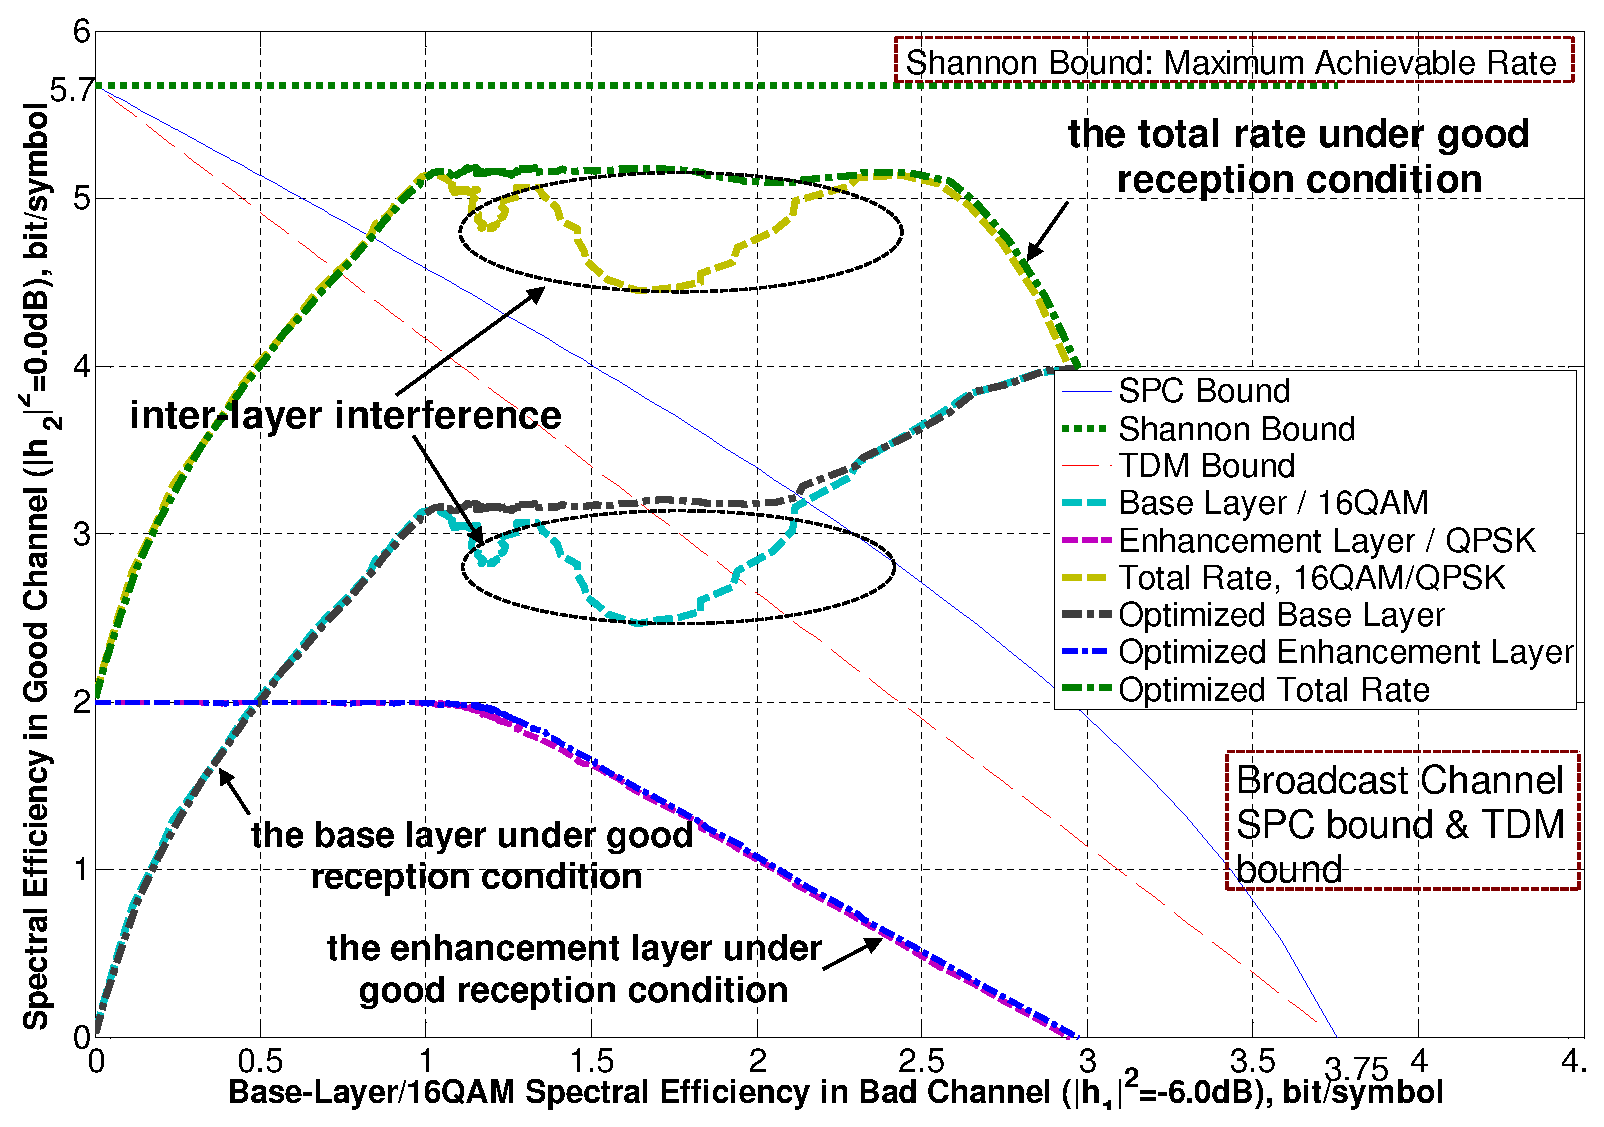
\includegraphics[width=3.0in, angle=0]{Capacity_100_025_16QAM.eps}
\caption{Achievable capacity of hierarchical modulations with
16QAM base layer and QPSK enhancement layer.}\label{Sum_Capacity}
}
\end{figure}
Hierarchical modulation is a signal precoding technique for
multiplexing multiple data streams into single symbol stream of
which each symbol consists of one base layer and one or multiple
enhancement layers. When signals of hierarchical modulation are
transmitted, users with good reception condition and advanced
receiver can demodulate multiple layers while others with poor
reception condition or conventional receiver may only demodulate
the data stream embedded in base layer. Therefore network operator
can target different types of users with different services. But
traditional hierarchical modulation may suffer from serious
inter-layer interference (ILI), where the achievable throughput by
low-layer signal(s), e.g. base-layer signals, is dented by
interference from high-layer signal(s). One example of this is
shown in Fig. \ref{Sum_Capacity}, where the 16QAM-modulated base
layer suffers from the existence of QPSK-modulated enhancement
layer. In order to recover the capacity loss due to the addition
of enhancement layer(s), two approaches are presented in this
paper. One approach is to rotate the signal constellation of
enhancement layer(s) so that higher capacity is achievable by
demodulating low-layer signals. The other one is to extend
traditional single-layer Gray mapping to multi-layer Gray mapping
for minimizing bit-error rate (BER). In Fig. \ref{Sum_Capacity},
it shows that the capacity loss by regular hierarchical modulation
can be restored by our proposed schemes. Partial of our schemes is
adopted in UMB by 3GPP2~\cite{UMB}.
\section{Sinal Model And Problem Description}
We will limit our discussions to two-layer signal constellations
with the enhancement layer QPSK-modulated and the base layer QPSK-
or 16QAM-modulated, although the concepts proposed here may be
generalized to most multi-layer hierarchical modulations. The
reason for this is not only because of the simplicity of QPSK and
16QAM modulations but also because QPSK and 16QAM are of the most
popular signal constellations adopted in various digital
communication systems and standards, and also the addition of QPSK
as enhancement layer may yield more significant performance gain
from our approaches. Furthermore, since many high-order regular or
hierarchical signal constellations may be decomposed into multiple
QPSK signals adding together, many analysis and conclusions
presented in this paper can be straightforwardly extended.

\begin{figure}
\center{
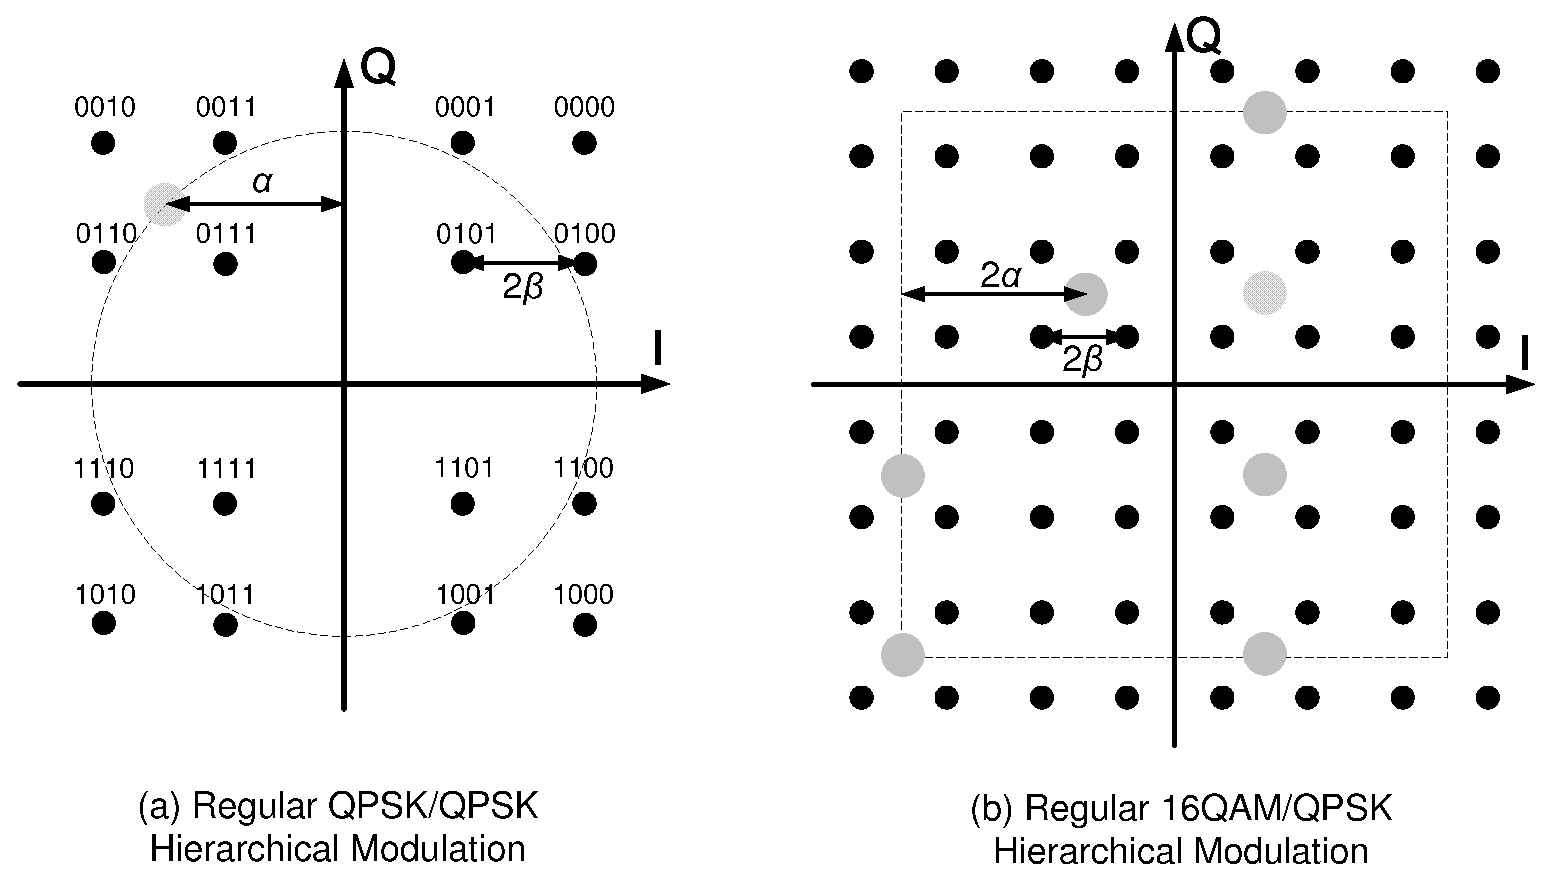
\includegraphics[width=3.0in, angle=0]{Regular_Hierarchical.eps}
\caption{Regular hierarchical modulation examples: the base layer
is QPSK/16QAM and the enhancement layer is
QPSK.}\label{regular_hierarchical} }
\end{figure}
The signal constellations of regular QPSK/QPSK and 16QAM/QPSK
hierarchical modulation are shown in Fig.
\ref{regular_hierarchical}. Obviously, a regular 16QAM can be
taken as a special case of QPSK/QPSK hierarchical modulation, in
which both base layer and enhancement layer are QPSK-modulated.
The minimum Euclid distance of base layer and enhancement layer
are denoted by $2\alpha$ and $2\beta$, individually. With
superimposing base-layer signal and enhancement layer signal
together, the minimum Euclid distance of resulted hierarchical
modulation becomes~\footnote{In this paper, we denote a
hierarchical signal constellation by the notation, {\em layer 0
constellation / layer 1 constellation / \ldots}, where the signal
constellation of different layers are separated by backslash from
the lowest layer (also called base layer ) to the highest layer. }
\begin{equation}
\begin{array}{rcccl}
d_{\rm min}& = & 2(\alpha-\beta) & <& 2\alpha
\end{array}.\label{Regular_MED}
\end{equation}
\noindent Smaller minimum Euclid distance usually results in more
ambiguity and higher demodulation BER. The bits-to-symbol mapping
of base-layer and enhancement-layer bits shown in
Fig.~\ref{regular_hierarchical} is a interleaved Gray mapping,
where the bits $b_{0}b_{1}$ from base layer and $e_{0}e_{1}$ from
enhancement layer are interleaved in one codeword
$b_{0}e_{0}b_{1}e_{1}$. The mapping shown in
Fig.~\ref{regular_hierarchical} for hierarchical signal
constellation can be taken as one-dimension Gray mapping, in which
the bits-to-symbol mapping rules of each layer are identical and
independent to each other. And this mapping is fixed regardless
the power-splitting ratio $\zeta$ between layers, which is defined
by
\begin{equation}
\begin{array}{rcl}
\zeta& = & \frac{P_{\rm E}}{P_{\rm B}}
\end{array}.\label{power_ratio}
\end{equation}
\noindent Usually $\zeta < 1$; otherwise we just think two signal
constellations exchanged positions in hierarchical signal
constellation. For QPSK/QPSK hierarchical modulation, the
power-splitting ratio is $\zeta_{\mbox{\tiny QPSK/QPSK}}=
\frac{\beta^{2}}{\alpha^2}$. For 16QAM/QPSK, $\zeta_{\mbox{\tiny
16QAM/QPSK}}= \frac{\beta^{2}}{4\alpha^2}$. When
$\zeta_{\mbox{\tiny QPSK/QPSK}}=\frac{1}{4}$, the regular
QPSK/QPSK modulation becomes rectangular-squared 16QAM.
Enhancement-layer signal can be taken as additional noise by the
base layer, especially when $\zeta$ is small. At this time, most
existing conventional receivers can continue to demodulate
base-layer signals at lower signal-to-noise/interference ratio
(SINR), which is written by
\begin{equation}
\begin{array}{rcccccl}
\hat{\gamma}& = & \frac{P_{\rm B}}{P_{\rm
E}+\sigma^2}&<&\gamma&=&\frac{P_{\rm B}}{\sigma^2}
\end{array},\label{SINR}
\end{equation}
\noindent even with no change on it. On the other hand, a new
advanced receivers can be designed to demodulate signals from both
base layer and enhancement layer(s). This is the feature that
makes hierarchical modulation attractive for providing seamless
upgrading, unequal protection, additional or differentiated
services with minimum changes on existing digital broadcast
systems. However, regular hierarchical modulation may seriously
suffer from ILI, which decreases not only the base-layer SINR
defined in (\ref{SINR}) but also its achievable rates. This is
shown in Fig.~\ref{Sum_Capacity} and more discussions of it will
be detailed in the rest of this paper. On the other hand, it is
well-known that the achievable throughput of a received signal
essentially depends on the power distribution profile of this
signal~\cite{Unge82}. From a channel coding point of view, higher
throughput is achievable by {\em i.i.d. Gaussian code}, even
though they may not be easily for implementation from an
engineering standpoint~\cite{Cover72}. How to transmit a signal
very close to Shannon channel capacity and implementable in a
relatively easy way is not only critical for the signal
constellation design block but also every other component in a
communication system.
\section{The Enhanced Hierarchical modulations}
In order to minimize ILI effect for higher achievable throughput,
we propose two approaches to enhance regular hierarchical
modulations, e.g., the one shown in
Fig.~\ref{regular_hierarchical}. The first approach is to
optimally rotate the enhancement-layer(s) of a signal
constellation. For the QPSK/QPSK hierarchical modulation shown in
Fig.~\ref{regular_hierarchical}, the QPSK signal constellation of
the enhancement layer is rotated in the anti-clock direction by
$\theta$, $0\leq\theta\leq\frac{1}{4}\pi$, and resulted signal
constellation is shown in Fig. \ref{enhanced_hierarchical}. With
optimal rotation angle $\theta_{\rm opt}$, most of the lost
base-layer capacity can be recovered without scarifying
enhancement layer(s). The achievable rates of 16QAM/QPSK
hierarchical modulations are plotted in Fig.~\ref{Sum_Capacity}.
\begin{figure}
\center{
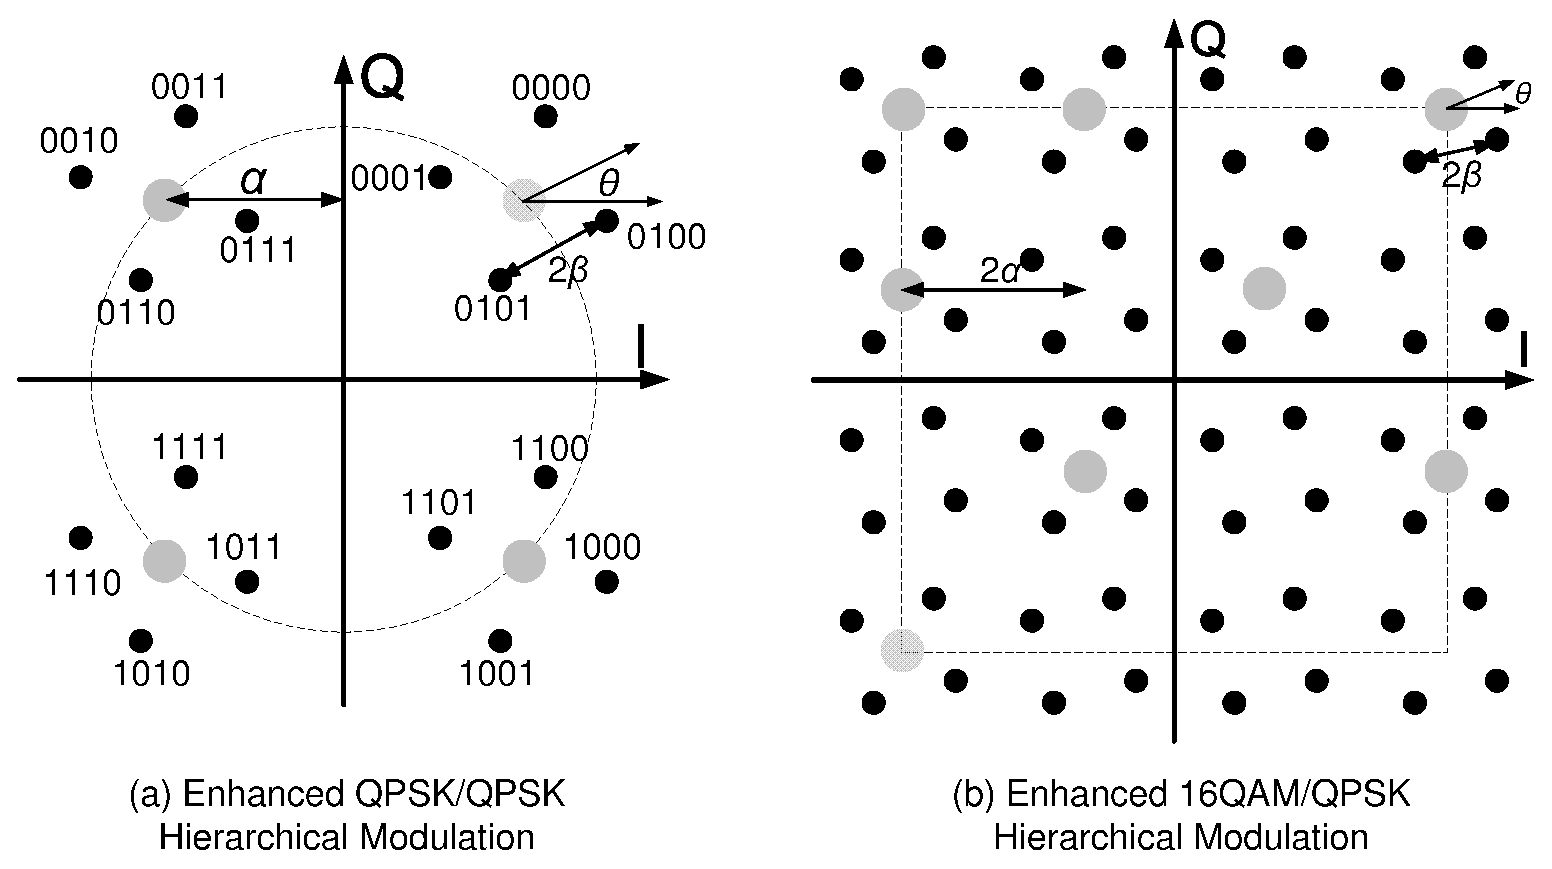
\includegraphics[width=3.0in, angle=0]{Enhanced_Hierarchical.eps}
\caption{Enhancing hierarchical modulation by rotating enhancement
layer.}\label{enhanced_hierarchical} }
\end{figure}

It is widely known that Shannon channel capacity is achievable
with Gaussian codes but it isn't implementable in reality. Most
existing capacity-achieving codes are designed to balance the
implementation complexity and performance. Gray code, also known
as reflective binary code, is a binary numeral system where two
successive value differ in only one digit. Even though it was
original designed to prevent spurious output from
electromechanical switches, Gray code for bits-to-symbol mapping,
mostly called Gray mapping, implemented with channel coding is
generally accepted as the optimal mapping rule for minimizing BER.
Gray mapping for regular QPSK/QPSK hierarchical modulation can be
found in Fig.~\ref{regular_hierarchical}, where the codewords with
minimum Euclid distance also have minimum Hamming distance.
However, the Euclid distance profile will change when the
enhancement-layer signal constellation is rotated as well as
power-splitting ratio is changed. This means the original Gray
mapping may not always be optimal. In this case, it may be
necessary to remap bits to symbols. One example of the Gray
remapping for QPSK/QPSK hierarchical modulation can be shown in
Fig. \ref{Gray_remapping}.
\begin{figure}
\center{
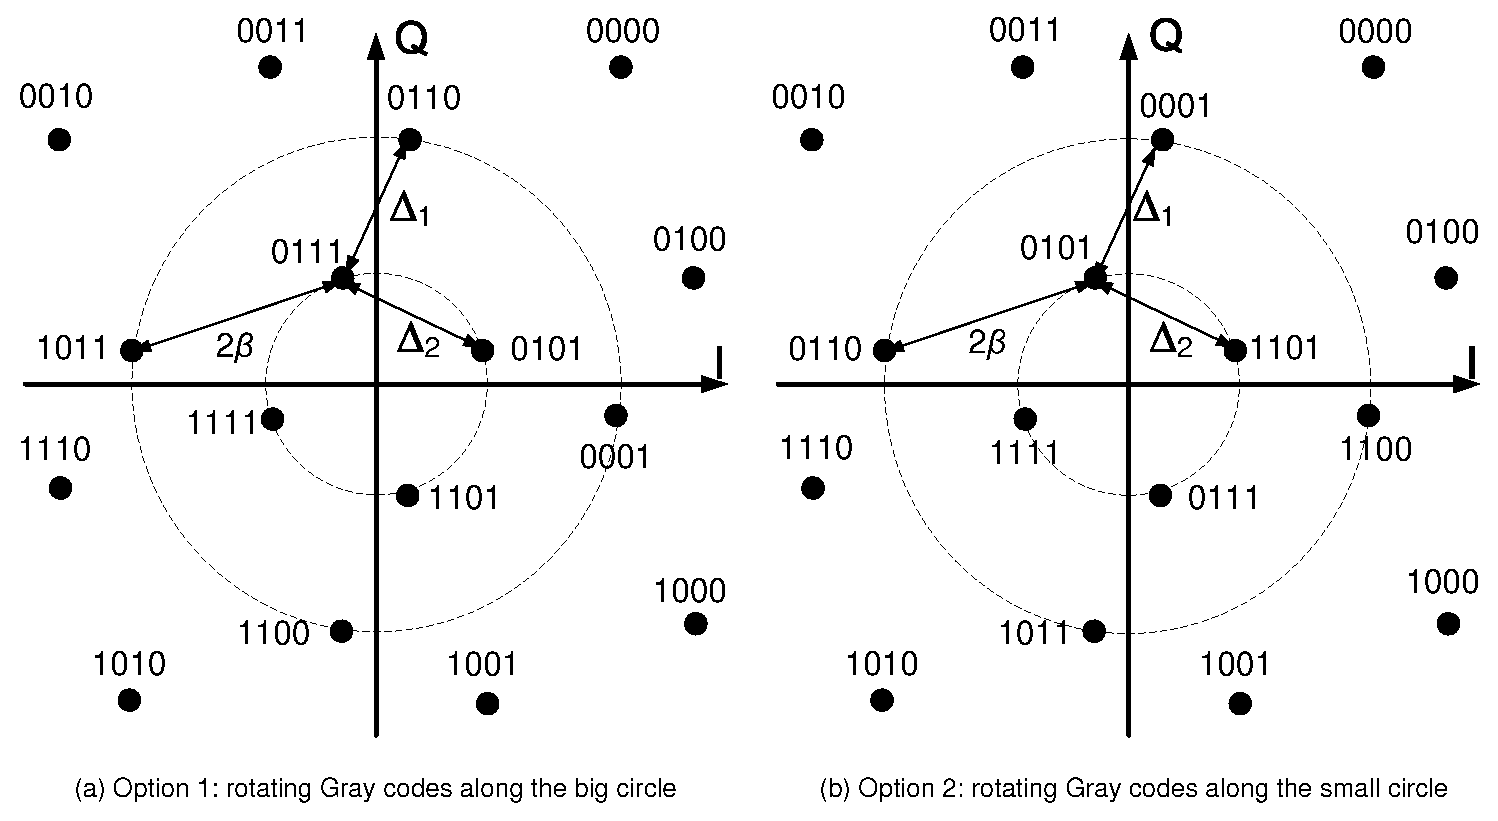
\includegraphics[width=3.2in, angle=0]{Gray_Remapping.eps}
\caption{Enhancing hierarchical modulation by multi-dimension Gray
mapping when $2\beta>\max\left\{\Delta_{1},\
\Delta_{2}\right\}$}\label{Gray_remapping} }
\end{figure}

In the following sections, we will detail the rationales behind
these two proposed approaches and also the discussion of their
performance. Computer simulation results are also provided to
support our analysis.
\section{Achievable Rates of Hierarchical Modulation~\label{Info_Theory}}
More three decades ago Cover showed that higher sum capacity is
achievable if messages for two users of different reception
conditions are superpositedly precoded~\cite{Cover72}.
Hierarchical modulation is one of the practical implementations of
superposition precoding (SPC) for providing different rates and
protections for users with different reception conditions. In
general, the achievable rate of a $N$-ary signal constellation,
either a regular signal constellation or a hierarchical signal
constellation, through AWGN channel can be calculated
by~\cite{Unge82}
\begin{equation}
\begin{array}{lcl}
R&=&\log_{2}\left(N\right)-\\
&&\hspace{-0.20in}\frac{1}{N}\sum\limits_{i=0}^{N-1}\mbox{E}\left\{\log_{2}\left[\sum\limits_{j=0}^{N-1}e^{-\frac{\left|s_{j}+n-s_{i}\right|^2-\left|n\right|^2}{2\sigma^2}}\right]\right\}\
,
\end{array}\label{N_ary}
\end{equation}
\noindent where $n$ denotes Gaussian white noise, which is real
with variance $\sigma^2$ and complex with variance $2\sigma^2$.
(\ref{N_ary}) is the achievable rate when a receiver try to decode
the whole hierarchically modulated symbol. With (\ref{N_ary}), the
AWGN capacity of regular QPSK and 16QAM can be plotted as in Fig
\ref{capacity_16QAM}. The rate indicated in (\ref{N_ary})
basically is achievable by users with advanced receiver. However,
for a user with a conventional demodulation receiver, it can
usually detect the base-layer signals and the rate of
(\ref{N_ary}) is more than what it can obtain. The actual
achievable rate should be lower than (\ref{N_ary}). Following the
concept of the successive interference cancellation proposed
in~\cite{Cover72}, the achievable rate, also termed {\em
equivalent capacity}, for a receiver decoding up to $l$ layers of
a hierarchical modulated symbol is~\footnote{A detailed treatment
of the concept {\em equivalent capacity} of hierarchical
modulation is out of the scope of this paper. It can be found
in~\cite{Huber94}. }

\begin{equation}
\begin{array}{rcccl}
\tilde{R}_{l}&=&\sum\limits_{i=0}^{l-1}R_{i}& = &
R-\sum\limits_{j=l}^{L}{R}_{j}
\end{array}.\label{R_equiv}
\end{equation}

\noindent Let's take a regular 16QAM as an example. A regular
16QAM can be take as a special case of QPSK/QPSK hierarchical
modulation with $\zeta=\frac{1}{4}$. With (\ref{R_equiv}), the
achievable rate of the enhancement layer is the same as regular
QPSK capacity. However, the achievable rate of the base layer
becomes

\begin{equation}
\begin{array}{rcl}
R_{\rm 16QAM}^{\rm B}\left(\gamma\right)&=&R_{\rm
16QAM}\left(\gamma\right) - R_{\rm QPSK}
\left(\frac{1}{5}\gamma\right)
\end{array}.\label{R_16QAM_B1}
\end{equation}

\noindent This can be shown in Fig \ref{capacity_16QAM}. Due to
the ILI from the QPSK enhancement layer, the actual throughput of
the QPSK base layer is lower than regular QPSK.

\begin{equation}
\begin{array}{rcl}
R_{\rm 16QAM}^{\rm B}\left(\gamma\right)&\leq&R_{\rm QPSK}
\left(\frac{4}{5}\gamma\right)
\end{array}.\label{R_16QAM_B2}
\end{equation}
\noindent The degradation of the base-layer capacity can be up to
around $\Delta=0.56$ bit/symbol, which is about $14\%$ of the
maximum total achievable capacity. This kind of degradation can be
further illustrated by Fig. \ref{capacity_rotating}. One of the
interesting things show in Fig. \ref{capacity_rotating}() is the
equivalent capacity of the 16QAM base layer is sort of
periodically instead of simple monotonically dented by ILI when
the percentage of the base-layer power increases. The good thing
is this kind of capacity loss may be recovered by properly
rotating the signals of enhancement layer.
\begin{figure}
\center{
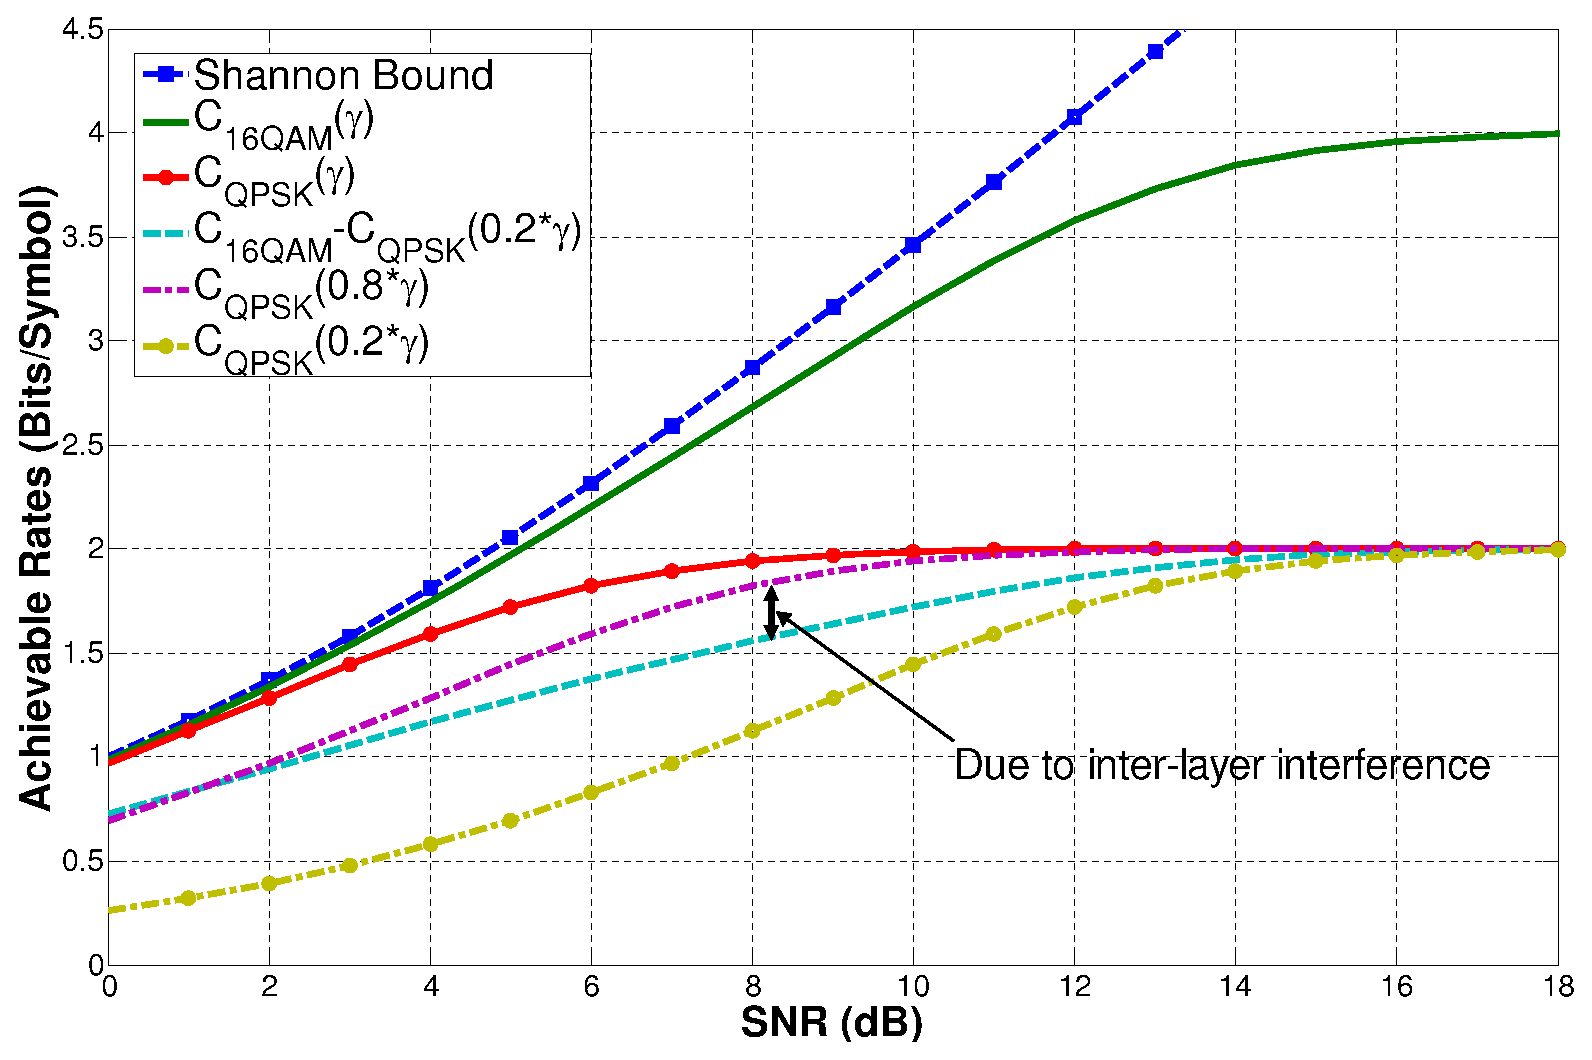
\includegraphics[width=3.0in, angle=0]{Capacity_16QAM.eps}
\caption{Achievable rates of regular 16QAM modulation: a
hierarchical modulation perspective.}\label{capacity_16QAM} }
\end{figure}

\begin{figure}
\center{
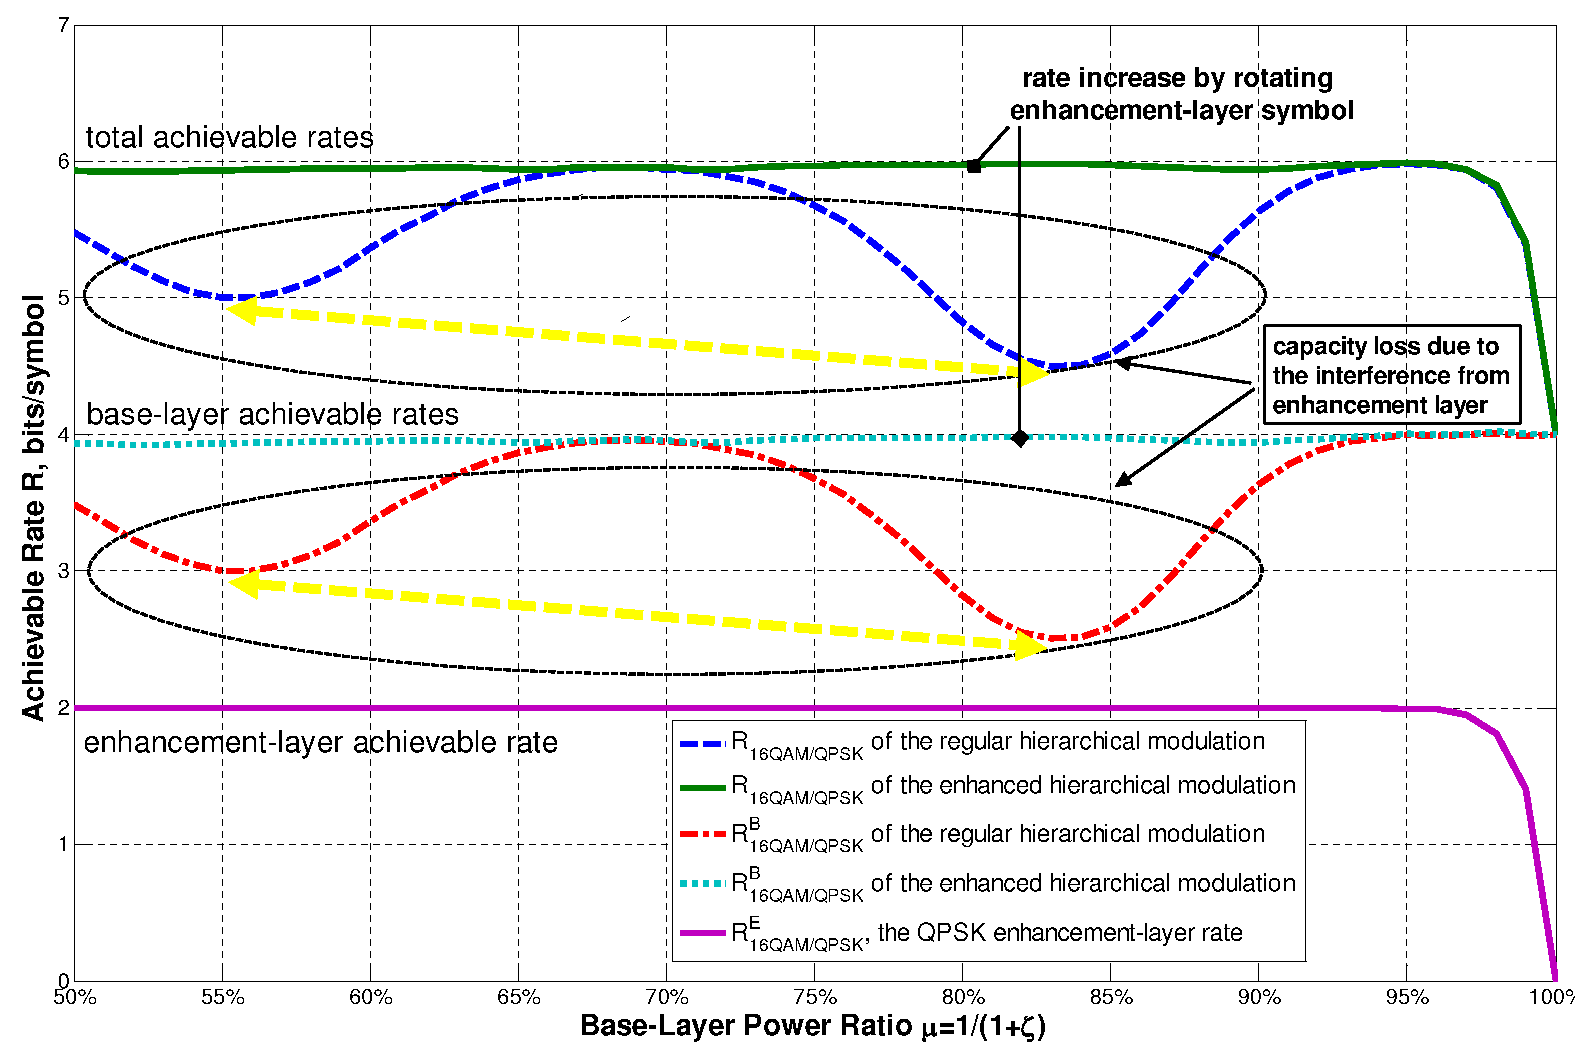
\includegraphics[width=3.0in, angle=0]{Capacity_power_splitting.eps}
\caption{Achievable rates of hierarchical modulations with
different power splittings. The base layer is 16QAM and the
enhancement layer is QPSK.
$\frac{P}{\sigma^2}=20$dB.}\label{capacity_rotating} }
\end{figure}

\section{Effective Signal-to-Noise Ratio and Modulation Efficiency}
Besides the information-theoretical point of view of hierarchical
modulation presented in Section~\ref{Info_Theory}, peoples are
also interested in understanding hierarchical modulation from a
signal-processing perspective. At this time, the performance of
hierarchical modulation will be evaluated through an actual
implementation and its demodulation BER is one of the major
concerns. In general, it is difficult to give a simple closed-form
BER expression for hierarchical signal constellation. The BER of
square-shaped $M$-QAM constellation and a hierarchical QAM
constellation can be recursively computed~\cite{Yang00,Vitt03}. It
is very well-known that the BER expression of QPSK is

\begin{equation}
\begin{array}{rcl}
P_{\rm
QPSK}\left(\gamma\right)&=&Q\left(\sqrt{\frac{\gamma}{2}}\right)
\end{array},\label{BER_QPSK}
\end{equation}
\noindent where $Q\left(\cdot\right)$ is the $Q$-function defined
by
\begin{equation}\hspace{-0.0in}
\begin{array}{rcl}
Q\left(x\right)&=&\frac{1}{\sqrt{2\pi}}\int\limits_{x}^{\infty}e^{-\frac{t^2}{2}}dt
\end{array}.\label{Q}
\end{equation}
%\noindent And the BER expression of a regular 16QAM is
%\begin{equation}
%\begin{array}{l}
%\hspace{-0.20in}P_{\rm
%16QAM}\left(\gamma\right)=\\
%\hspace{0.10in}\frac{1}{4}\left[3Q\left(\sqrt{\frac{\gamma}{5}}\right)+2Q\left(3\sqrt{\frac{\gamma}{5}}\right)-Q\left(\sqrt{5\gamma}\right)\right]\
%.
%\end{array}\label{BER_16QAM}
%\end{equation}

\begin{figure}
\center{
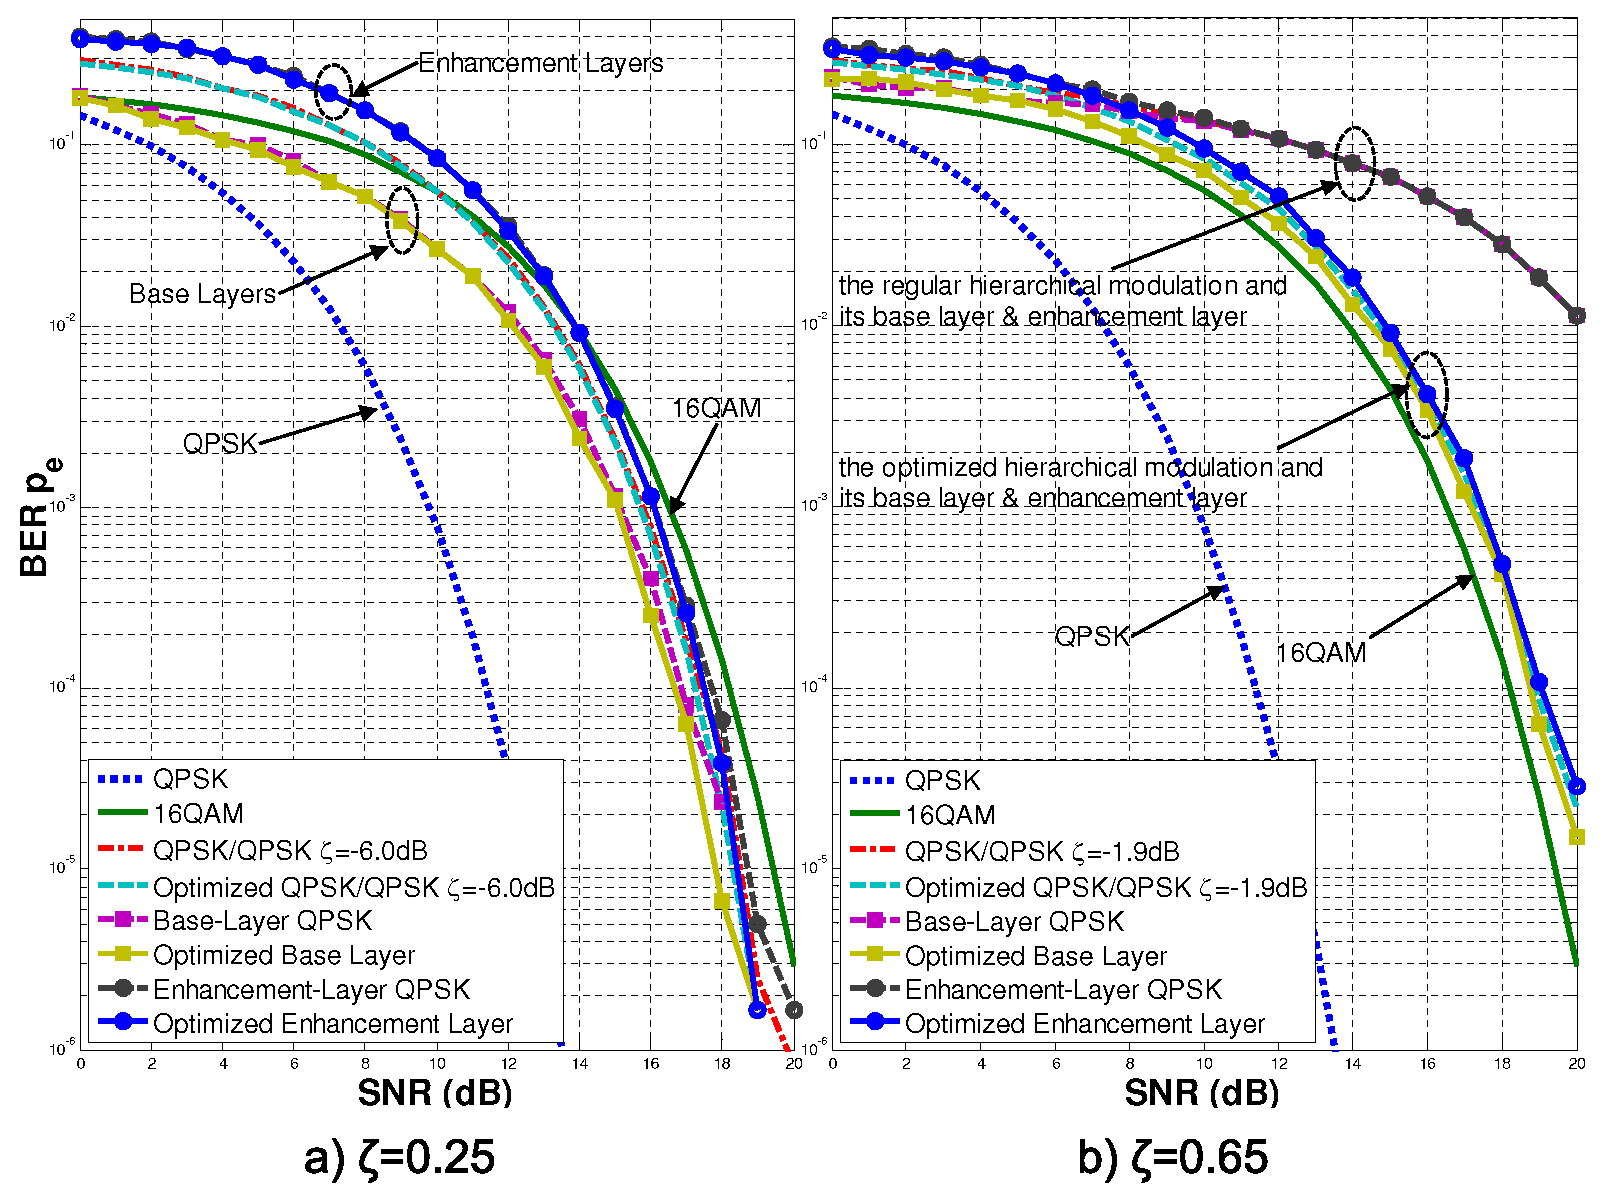
\includegraphics[width=3.20in, angle=0]{BER_Hierarchical.eps}
\caption{Bit-error rate of uncoded QPSK/QPSK hierarchical
modulations using maximum likelihood demodulation . } \label{BER}}
\end{figure}

From signal processing point of view, the BER and capacity
degradation possibly happen when there is a change in noise and/or
interference distribution(s), even though the received SNR
$\gamma$ and the receiver are the same. This is shown in Fig.
\ref{BER}. When $\zeta$ increases, BER performance of regular
QPSK/QPSK hierarchical modulation becomes deteriorated. However,
if we properly rotate the enhancement-layer signal constellation,
this performance loss can be recovered. This kind of recovery can
be significant when $\zeta$ is large. There are many ways
quantifying this kind of BER performance loss due to interference
and receiver design. One approach for capturing this kind of
degradation is to calculate the effective signal-to-noise ratio
(ESNR) of the receiver output, which is defined by

\begin{equation}
\begin{array}{rcl}
\tilde{\gamma}&\equiv&\Psi^{-1}\left(p_{e}\right)
\end{array},\label{eff_SNR}
\end{equation}

\noindent where $p_{e}$ is the demodulation BER of the signal with
actual SNR $\gamma=\frac{P}{\sigma^2}$, and
$\Psi^{-1}\left(\ast\right)$ denotes the inverse function of
$\Psi\left(\cdot\right)$, which denotes the error probability
function of demodulating the signal in AWGN channel. With
(\ref{BER_QPSK}), the ESNR of a QPSK-modulated base layer or
enhancement layer can be calculated by
\begin{equation}
\begin{array}{rcl}
\tilde{\gamma}_{\rm
QPSK/QPSK}&=&2\left[Q^{-1}\left(p_{e}\right)\right]^2
\end{array}.\label{eff_SNR_QPSK}
\end{equation}
\noindent With normalizing ESNR by actual SNR, we can define
hierarchical modulation efficiency $\eta$ by

\begin{equation}
\begin{array}{rcccl}
\eta\left(\gamma\right)&=&\frac{\tilde{\gamma}}{\gamma}&=&\frac{1}{\gamma}\Psi^{-1}\left(p_{e}\right)
\end{array}.\label{mod_eff}
\end{equation}

\noindent When there is no interference and a maximum likelihood
demodulator is used, $\eta\left(\gamma\right)=1$; Otherwise,
$\eta\left(\gamma\right)<1$.  The asymptotic modulation efficiency
$\eta_{\infty}$ is given by

\begin{equation}
\begin{array}{rcccl}
\eta_{\infty}&=&\lim\limits_{\gamma\rightarrow\infty}\eta\left(\gamma\right)&=&\lim\limits_{\sigma\rightarrow0}\frac{\sigma^2}{P}\Psi^{-1}\left(p_{e}\right)
\end{array}.\label{asy_mod_eff}
\end{equation}
\noindent The modulation efficiencies of QPSK/QPSK hierarchical
modulations are plotted in Fig. \ref{modulation_efficiency}. We
can see that the enhanced hierarchical modulation has higher
modulation efficiency than the regular modulation. Especially when
$\zeta$ is larger, the difference is more obvious.

\begin{figure}
\center{
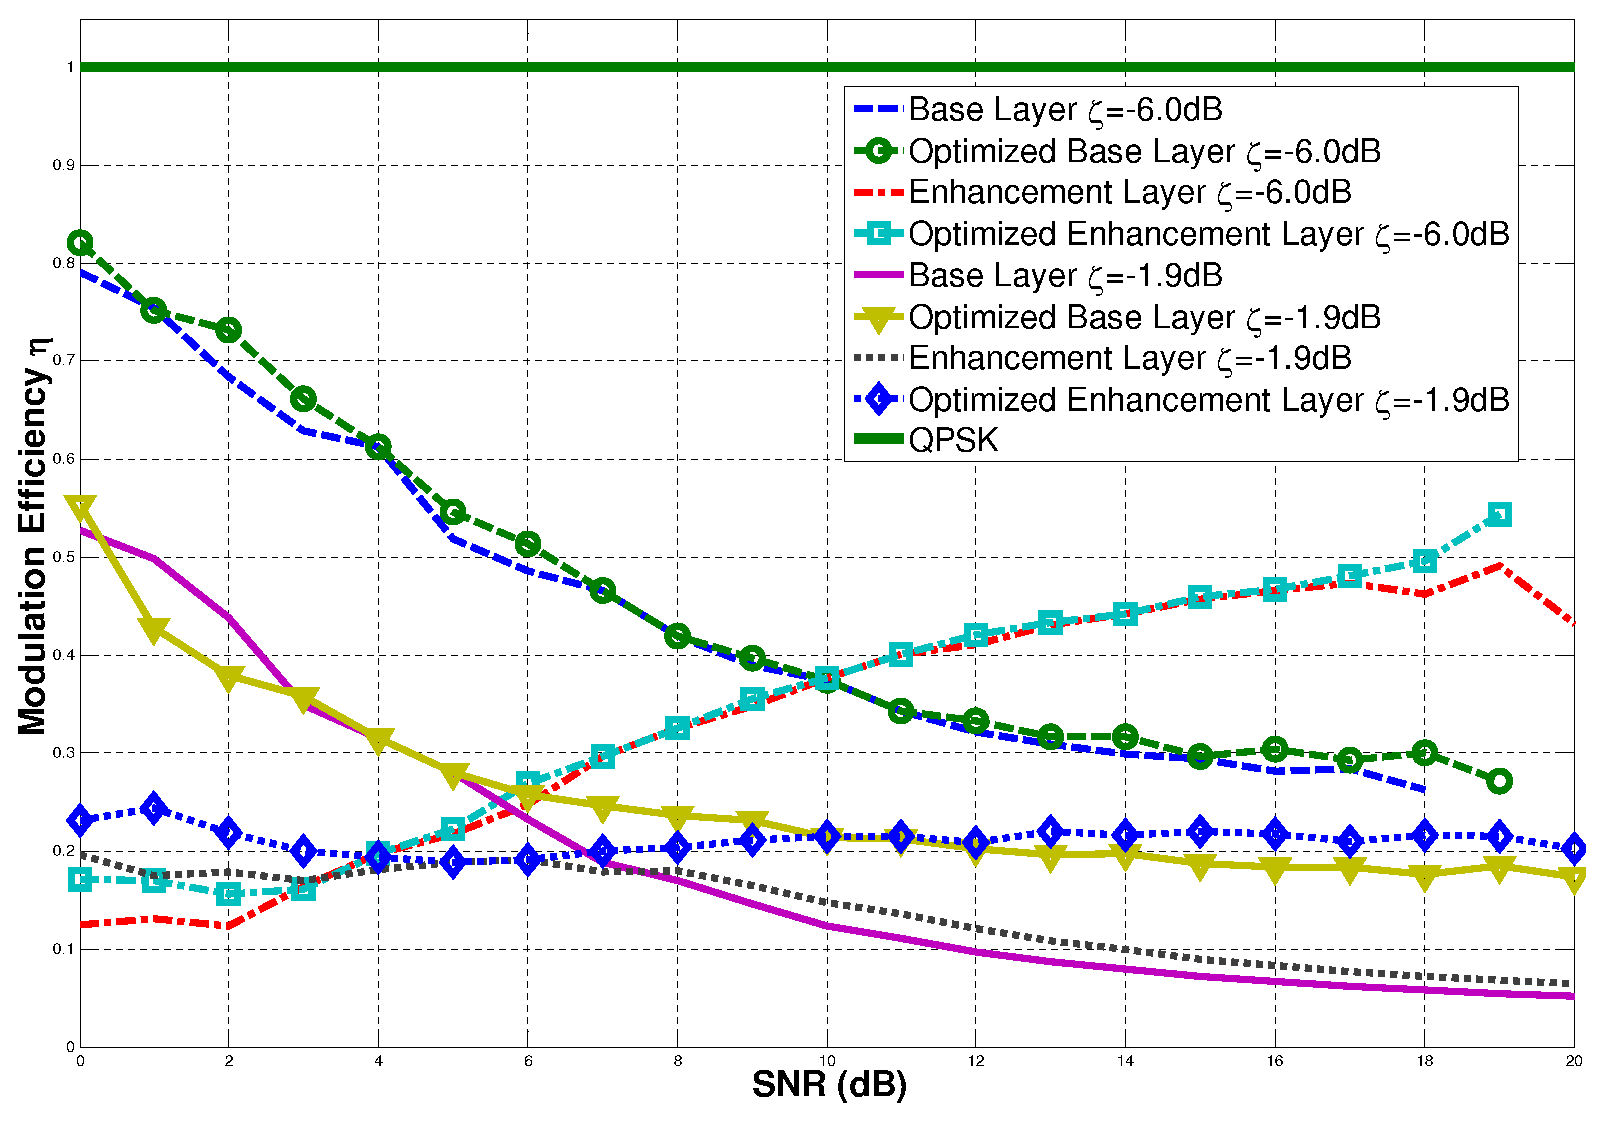
\includegraphics[width=3.0in, angle=0]{Modulation_Efficiency.eps}
\caption{Hierarchical modulation efficiency of QPSK/QPSK
hierarchical modulation using maximum likelihood
demodulation.}\label{modulation_efficiency} }
\end{figure}

\section{Euclid Distance and Hamming Distance}
When a receiver select $\bs_i$ instead of the transmitted symbol
$\bs_j$, there is a demodulation error happened. The demodulation
error for AWGN channel is

\begin{equation}
\begin{array}{rcl}
Pr\left(\bs_{j}\rightarrow\bs_{i}|\bs_{j}\right)&=&Q\left(\frac{\|\bs_{i}-\bs_{j}\|}{\sqrt{2}\sigma}\right)
\end{array}.\label{prior_error}
\end{equation}

\noindent In general case of a Rician fading channel with
Rice-Factor $K$, the chernoff upper bound of
$Pr\left(\bs_{j}\rightarrow\bs_{i}|\bs_{j}\right)$ is given by

\begin{equation}
\begin{array}{ll}
\hspace{-0.2in}Pr\left(\bs_{j}\rightarrow\bs_{i}|\bs_{j}\right)&\\
&\hspace{-0.8in}\leq\
\frac{1+K}{1+K+\frac{1}{2}\gamma\|\bs_{i}-\bs_{j}\|^2}e^{-\frac{K\frac{1}{2}\gamma\|\bs_{i}-\bs_{j}\|^2}{1+K+\frac{1}{2}\gamma\|\bs_{i}-\bs_{j}\|^2}}\
.
\end{array}\label{prior_error_fading}
\end{equation}


\noindent The BER performance of a signal constellation is
dominated by symbol pairs with small Euclidean distance $d_{\rm
min}$. An example of the minimum Euclidean distance of
hierarchical distance with rotating enhancement layer can be shown
in Fig.~\ref{euclid_dist}.

In general, Gray mapping in two-dimensional signals is accepted as
optimal for minimizing BER for equally likely signals. Gray
mapping for regular hierarchical signal constellations is shown in
Fig.~\ref{regular_hierarchical}, where the codes for the closest
two signals are different in only one bit. However, this kind of
Euclidean distance profile may not be fixed in hierarchical
modulation. For example, when the power splitting ratio $\zeta$
increase in a two-layer hierarchical modulation, the Euclidean
distance between the base-layer signals and the enhancement-layer
signals changes too and the distance of some previous closest
signal pairs may be not the shortest any more. This may also
happen when the enhancement layer is rotated. Therefore in order
to minimize BER when Euclidean distance profile is changed in
hierarchical modulation, it may be necessary to do Gray-remapping.
One example of Gray remapping is shown in
Fig.~\ref{Gray_remapping}. Their BER performance is shown in Fig.

% \begin{equation}
% \begin{array}{rcl}
% P_{e}&=&\sum\limits_{i\neq j}Pr\left(\bs_{j}\rightarrow\bs_{i}|\bs_{j}\right)Pr\left(\bs_{j}\right)\\
% &\leq&Q\left(\frac{d_{\rm min}}{\sqrt{2}\sigma}\right)
% \end{array}.\label{error}
% \end{equation}


\begin{figure}
\center{
\includegraphics[width=3.0in, angle=0]{MED_16QAM_QPSK.eps}
\caption{Minimum Euclidean distance of 16QAM/QPSK
modulations}\label{euclid_dist} }
\end{figure}



\section{Conclusions}
In this paper, two schemes for enhancing hierarchical modulations
are presented for higher throughput and less error rate. One
approach is to optimize the signal constellation and the other one
is to do multi-dimensional Gray mapping. The rationale and
performance of the proposed approaches are discussed and analyzed
by calculating the achievable rate, effective signal-to-noise
ration and minimum Euclidean distance. These two approaches can be
applied for upgrading existing broadcast systems with minimum
complexity increase and designing the next-generation BCMCS
systems. Some of them is adopted in the 4th generation mobile
communication standard UMB by 3GPP2.

\small
\bibliographystyle{unsrt}
\bibliography{Hierarchical_Modulation}
\end{document}
